\documentclass{kththesis}

\usepackage{graphicx}
\usepackage{todonotes}
\usepackage{blindtext} % This is just to get some nonsense text in this template, can be safely removed

\usepackage{csquotes} % Recommended by biblatex
\usepackage[style=numeric,sorting=none,backend=biber]{biblatex}
\addbibresource{references.bib} % The file containing our references, in BibTeX format

\title{Comparison of Progressive Web Apps and Native Android Application}
\alttitle{Detta är den svenska översättningen av titeln}
\author{Camille Fournier}
\email{camillef@kth.se}
\supervisor{Javier Cabrera-Arteaga}
\examiner{Benoit Baudry}
\hostcompany{Odiwi} % Remove this line if the project was not done at a host company
\programme{Master in Computer Science}
\school{School of Electrical Engineering and Computer Science}
\date{Spring 2020}

% Uncomment the next line to include cover generated at https://intra.kth.se/kth-cover?l=en
% \kthcover{kth-cover.pdf}

% Commands
\newcommand{\citationneeded}{\todo{Citation needed}[!]}
\newcommand{\red}[1]{{\color{red} #1 }}

\begin{document}
\sloppy % prevent non cut in large url


% Frontmatter includes the titlepage, abstracts and table-of-contents
\frontmatter

\titlepage

\begin{abstract}
  English abstract goes here.

  \blindtext
\end{abstract}


\begin{otherlanguage}{swedish}
  \begin{abstract}
    Träutensilierna i ett tryckeri äro ingalunda en oviktig faktor,
    för trevnadens, ordningens och ekonomiens upprätthållande, och
    dock är det icke sällan som sorgliga erfarenheter göras på grund
    af det oförstånd med hvilket kaster, formbräden och regaler
    tillverkas och försäljas Kaster som äro dåligt hopkomna och af
    otillräckligt.
  \end{abstract}
\end{otherlanguage}


\tableofcontents


% Mainmatter is where the actual contents of the thesis goes
\mainmatter


\chapter{Introduction}

\todo[inline]{Introduction for late writing}
\todo[inline]{Section names as questions is not good :)}
\todo[inline, color=cyan!20]{What title would be good then ? Because we should have a section specific for the research questions right ?}

\indent 

One of the biggest challenge of mobile development today resides in the high fragmentation of mobile platforms \cite{MobileDevChallenges} with developers building the same app over multiple platforms. A popular solution is cross-platform development, that is using a framework capable of using the same code for multiple platform builds.  However, such cross-platform development does not concern web applications that developers still have to develop separately from mobile applications. To answer this problem, Google introduced in 2015 the concept of \textit{Progressive Web Apps} \cite{PWA_intro}, a term first coined by designer Frances Berriman and Google Chrome  developer Alex Russel \cite{PWA_blog} \cite{PWApossibleUnifer}.
This section will introduce the concept of Progressive Web Apps and the objective of this paper.

\section{Why is it beneficial ?}
\todo[inline, color=cyan!20]{Cite papers describing PWAs success stories, benefits and importance of bringing web to mobile}
\todo[inline]{Move to Methodology}
\todo[inline, color=cyan!20]{Why to Methodology ? Maybe background instead, in Literature ?}


\section{Research Questions}

Due to its cross-platform capabilities, Progressive Web Apps seems like a promising alternative to native development. However, this shouldn't come at the cost of app performance and user experience, especially in regards to smoothness.
Thus, this paper will aim at answering the question : 
\begin{center}
    \textit{Can Progressive Web Apps be as smooth as Mobile Applications ?}
\end{center}
Which raises the following sub-questions: 
\begin{enumerate}
    \item What metrics are relevant to compare the smoothness of Mobile and Progressive Web Apps?
    \item What tools are available to measure those metrics ?
\end{enumerate}

\section{Limitations}

Every research paper comes with its limitation, and this paper is no exception. 
At the time of writing, Progressive Web App are not fully supported on iOS \cite{BackgroundSync_support} \cite{Manifest_support}. Thus, this paper will focus on comparing PWA and traditional mobile applications only on Android. 
Moreover, according to Statcounter \cite{Browser_data} which compiles data from more than 10 billion page views per month, the browser used on mobile the most is Google Chrome with more than 60\% usage followed by Safari with 26\% and other browsers at less than 10\%. 
Considering the overwhelming usage of Google Chrome on Android devices, this paper will focus on PWA's performance with Google Chrome. 



\chapter{Background}

%\todo[inline]{Every chapter should have a summary introduction. What is this chapter about?... For example, In this chapter we talk about Android application development, profiling tools...}

%\todo[inline]{Write here every needed background, for example, what is an emulator? etc}

This chapter presents the terminology and concepts related to this study, as well as previous research done on Progressive Web Apps and available tools to measure Android apps and PWA's performance.  

\section{Mobile applications}
\subsection{Development}
There is a number of ways to develop a mobile application today. One of the most common approach is to develop it natively, that is develop the mobile application once for each targeted platform (mainly iOS, Android) using their respective environment, Software Development Kit and programming language. Since this can be quite costly, an alternative has emerged in the form of cross-platform development. It is itself divided in several different approaches implemented by different frameworks. Such approaches share a common characteristic: the use of the same code to build the application for several platforms. 
Traditionally, cross-platform development is divided into four different approaches \cite{CrossPlatform_dev} :
\begin{itemize}
    \item Web : The web app is run by the browser on the mobile device. PWAs are an improvement of this approach
    \item Hybrid : The application is built using web technology but executed inside a native container. The app is rendered through full screen web-views. Frameworks like PhoneGap and Ionic \cite{crossplatform_approaches} use this approach.
    \item Interpreted : The application code is ran by an interpreter which uses native components to create a native user interface. Frameworks like React Native, NativeScript and Titanium \cite{emulating_native_w_crossplatform} use this approach.
    \item Cross-Compiled : The source code is compiled into a native application by a cross-platform compiler. Xamarin \cite{crossplatform_approaches} uses this approach. 
\end{itemize}


\subsection{Emulators}
    It is considered a largely accepted best practice to test an under development before production. This can be done using physical devices or emulators. An emulator is a software that simulates the software and hardware capabilities of a device\cite{emulator_def}. This can be a great way to automate testing among a large range of smartphones. Most of the Android emulators found during this research are targeted are gamers and enhance the hardware capabilities usually found in the simulated physical device. Only a few can be used by developers to test the performance of their applications among different smartphones.
    
\paragraph{}
\textbf{Android Emulator} \cite{android_emulator} is the official emulator for Android provided by Google along Android Studio. It offers the latest Android APIs but a limited range of physical devices. However, it is possible to customize hardware characteristics and the device's look.

\paragraph{}
\textbf{Genymotion} \cite{genymotion_emulator} contains a wider range of smartphones but less APIs than Android Emulator. Genymotion can be linked with Android Studio in order to test in-development apps. It is also possible to customize hardware characteristics.

\paragraph{}
\textbf{Visual Studio Android Emulator} \cite{microsoft_emulator} is the solution offered by Microsoft on Visual Studio. However, it is not supported since Visual Studio 2017 and recommend instead to use the official Android Emulator. It offers a limited set of hardware and API configurations that matches several smartphones at once. 

\section{Progressive Web Apps}

\subsection{Concept}

A Progressive Web , or PWA in short, is a regular web application with a few more features. Its aim is to reduce the gap between mobile and web development. Once it is installed, a PWA should behave just like a native app for the end-users. Thus, they should not be aware of the browser running the app behind the scene, and be able to launch the app without internet connectivity. \newline
The concept of Progressive Web Apps holds a lot of potential \cite{PWApossibleUnifer}. It could allow developers to use the same code for the web, the mobile, and the desktop app depending on browser implementations. This would considerably reduce the development and maintenance cost of a single application. Moreover, deployments and updates wouldn't have to go through the app stores to be available to users, further reducing the cost and increasing access to the app.
\paragraph{}
In order to be called a Progressive, a web application has to implement several features\cite{PWA_def}:
\textendash
%\renewcommand{\labelitemi}{$\textbullet$}
%command doesn't work for unknown reason
\begin{itemize}
    \item \textbf{Progressive:} Work for every browser
    \item \textbf{Responsive:} Fit any screen size
    \item \textbf{Connectivity independent:} Able to work offline or with low-connectivity thanks to a service worker
    \item \textbf{App-like:} Have a Native-like interaction by using the app-shell model
    \item \textbf{Fresh:} Keep the app up-to-date with the service worker
    \item \textbf{Safe:} Served over TLS to prevent snooping and content tampering
    \item \textbf{Discoverable:} Identifiable as "applications" thanks to W3C manifests and service workers
    \item \textbf{Re-engageable:} Use re-engagement features like push-notifications
    \item \textbf{Installable:} Save the app on the home screen without going through an app store
    \item \textbf{Linkable:} Share the app with a simple URL
\end{itemize}
\todo[inline]{Separate in another subsection: "Architecture", for example. Maybe is a good idea to have a diagram...next iteration}

\subsection{Architecture}

In practice, Progressive Web Apps contains 3 main components : the web app manifest, the service worker and the app shell (see figure ).

\medskip
\textbf{App Manifest} \newline
The web app manifest is a JSON file containing the metadata concerning the native display of the app once installed on the user's phone. In this file, the developer can define the app's metadata such as the splash screen, the app icon, the theme color and the app title. Without it, the app is uninstallable.

\medskip
\textbf{Service Worker} \newline
The service worker is the central part of a PWA. It is responsible for the new background features such as push notifications, offline experience and background synchronization\cite{SW_def}. The service worker acts as a proxy server for the PWA: it intercepts requests, cache the response or give the already cached response. As a worker, it doesn't have access to the DOM and works on a different thread as the main app. 

\medskip
\textbf{App shell} \newline
The app shell is essentially the User Interface of the app without any content \cite{AppShell_def}. By caching it via the service worker, it offers the user a better performance with instant loading of the UI on repeat visits and a better low-connectivity experience.


\subsection{Academic Research} 
%\todo[inline, color=orange!40]{Related work?}

%\todo[inline, color=orange!40]{No more than 6 sentences per cite in related work. Relevant work, limitations and differences with this thesis}

Though Progressive Web Apps have sparked a real interest in the mobile and web development industry, only a few research papers studied them\cite{PWApossibleUnifer} \cite{Biorn-Hansen2} \cite{Biorn-Hansen3}.
\paragraph{}
When studying performance, a large portion of the researched papers focused on the app start-up times. They measured either the total launch time\cite{YbergViktor2018NPaU} \cite{PWApossibleUnifer} \cite{Biorn-Hansen2}, the time from app-icon to toolbar render \cite{PWApossibleUnifer} \cite{Biorn-Hansen2}, the first paint \cite{bac_pwa_comparison} \cite{bac_pwa_performance} \cite{PWAapplicability} or other metrics related to start up \cite{bac_pwa_performance} \cite{bac_pwa_comparison}.
Their results showed that the launch time was faster for a PWA than a mobile app when the browser was already in memory. The app icon from toolbar render as well as the first paint metrics also showed that PWA was one of the fastest among the apps tested.\newline
Only one study concluded that PWA was slower was slower than a regular web app because of the HTTPS requests \cite{bac_pwa_comparison}. However, the comparison was made between a PWA served over HTTPS and a regular web app served between HTTP. Another other study \cite{bac_pwa_performance} which also compared a regular web and a PWA First Paint time did not find such results. 

\paragraph{}
Two research papers also investigated the energy consumption of PWA, though from a different angle. Malavolta et al.\cite{SW_and_energy} focused on the impact of service workers on PWA's energy consumption and found no significant significant impact. Kerssens \cite{PWAapplicability} on the other hand measured the average energy consumption when running the app and found PWA consumes slightly less than its native counterpart. 

\paragraph{}
Fransson and Driaguine \cite{PWAbc_responsetime} compared the response time of PWAs and Native Android Applications when accessing the camera en geolocation. The Progressive Webb App was surprisingly faster at using geolocation than its native counterpart. However, the camera was accessed faster from the native app than the PWA.

\paragraph{}
Lee et al. \cite{Pride_Prejudice} explored the security system behind the push notification system for Progressive Web Apps and found several concerning flaws which they reported to the vendors. 

\paragraph{}
Lastly, only two research papers examined the user experience offered by Progressive Web Apps. Cardieri and Zaina \cite{PWA_UX_comparison_study} conducted a qualitative analysis of user experience on three platforms: web mobile, native android and PWA. They concluded that there was no significant difference of user experience between the platforms. Fredrikson \cite{emulating_native_w_crossplatform} also supports this conclusion with a quantitative and a qualitative study comparing user experience with a React Native App, a Native Android App and a Progressive Web App. 

\section{Profiling tools}

Profiling tools are software or command-line tools that help developers evaluate the performance of their app or identify performance bottlenecks. They can measure metrics such as \%CPU, the memory used or functions called during a recording.
This section introduces several profiling tools for Android and Web applications.



\subsection{Android}

Not many tools are available to profile Android applications aside from Android Profiler \cite{nanoscope}. This software can provide real-time information about CPU, Memory, Network and Battery consumption in the form of graphs. While it does not require any specific install as it comes with Android Studio and provides a User Interface, it can have a high overhead \cite{nanoscope} and make the app less performant during recording than it usually is. 

\paragraph{}
Fortunately, Android also provides other command-line tools to profile applications. Most of them are only available through Android Debug Bridge (ADB) \cite{adb} which allows a computer to communicate with a device either to get information or execute commands. 

\paragraph{}
For example, dumpsys \cite{dumpsys} can provide a lot of information about the device or the processes currently running. This information is available through the system services such as \textit{meminfo} (memory), \textit{cpuinfo}, \textit{gfxinfo} (animation), \textit{netstats} (network) or \textit{batterystats} (battery).

\paragraph{}
Another example is top. It comes from the Linux command-line of the same name \cite{top}, but with limited options. It displays the process activity in real-time such as CPU, memory and priority.

\paragraph{}
Systrace \cite{systrace} is also a useful tool and does not require ADB. It records a device activity and outputs an HTML file which can be viewed on Chrome browser. This file displays a timeline of events for each threads running during the recording, the CPU activity divided for each CPU, frames and other events depending on the categories of events selected. It is mainly used to identify the cause of bottlenecks in an application.

\paragraph{}
While not a profiling tool in itself, Monkeyrunner \cite{monkeyrunner} is a useful tool when testing an application. Its purpose is to automate testing by interacting with the device from a Python script. It can also take snapshots or execute \textit{adb shell} commands, such as dumpsys and top viewed previously. 

\subsection{Progressive Web App}

As Progressive Web Apps are after all web applications that runs on the browser, many of the tools available depends on the browser running the app. Thus, the tools presented here may only apply to apps running on Chrome.

\paragraph{}
One of them is Chrome DevTools, a complete set of developer tools available in Chrome Browser. It is divided into several panels each with its own purposes. For example, the \textit{Network} panel displays all requests done by the web app, the \textit{Console} panel displays debug and error messages and the \textit{Performance} panel \cite{chrome_devtools_perf} displays an overview of the app performance, such as a timeline of function calls, a CPU graph, a memory graph and information regarding frames. 

\paragraph{}
Lighthouse \cite{lighthouse} is another tool of Chrome DevTools, available in the \textit{Audit} panel. Though its purpose is to automatically assess any web page's quality (Best Practices, performance, Search Engine Optimization, Accessibility,, Progressive Web App), its main target are Progressive Web Apps \cite{PWApossibleUnifer}. 

\paragraph{}
Chrome DevTools Protocol \cite{CDP} is a set of commands and events used to communicate with the browser and the web page. Chrome DevTools takes its source of information from it. A number of other tools relies on it for their features \cite{awesome_CDP}. It may be used for browsers other than Chrome if they are based on Blink.



\section{Rendering Pipeline}

\todo[inline, color=orange!40]{Maybe a quick introduction for this section. "Why is important to know how the rendering pipeline works?"}
The smoothness of an application greatly depends on the frame rate. The faster an app can produce a new frame, the faster it can display a response to user input and the more animations it can properly handle without blocking the user interaction. \newline
Though the goal of Progressive Web Apps is to look and behave the same as mobile application once installed on a smartphone, they rely on different technologies to do so. Thus, the rendering pipeline (the stages by which a frame is produced) can differ.


\subsection{Android}

The Android Graphics pipeline is divided between 3 main components: the Application Renderers, SurfaceFlinger and the Hardware Composer \cite{android_graphics}.
When an application wants to display something on the screen, its Application Renderer (usually provided by Android framework) gives a buffer of graphical data to SurfaceFlinger. SurfaceFlinger then takes all available buffers and composes them into a single buffer that it passes on to the Hardware Composer (see figure \ref{fig:android_data}). The Hardware Composer is responsible for actually displaying the buffer on the screen.
\newline

\begin{figure}[!ht]
    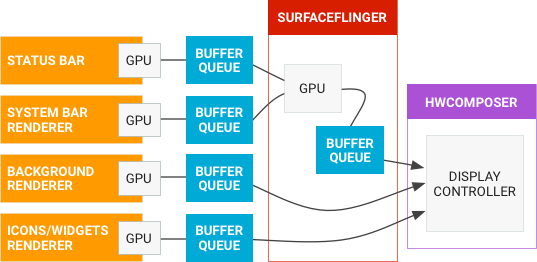
\includegraphics[width=13cm]{kththesis/Figures/android_data_flow.png}
    \caption[Graphic data flow through Android]{Graphic data flow through Android \footnotemark}
    \label{fig:android_data}
\end{figure}

\footnotetext{Source: \url{https://source.android.com/devices/graphics}}

Everything displayed on the screen have to go through SurfaceFlinger and the Hardware Composer.
All these components synchronize with each other thanks to the VSYNC signal \cite{vsync}. When VSYNC signal is fired, all three components wake up : the App Renderers generates frame N, SurfaceFlinger takes a look inside the BufferQueue and composes frame N+1 if a new buffer is available, and the Hardware Composer displays frame N+2. The VSYNC signal depends on the device refresh rate, usually set at 60Hz though some new devices also support 90 or 120Hz \cite{refresh_rate}.

\paragraph{}
Application rendering itself is divided into 7 different stages \cite{app_rendering}:
\begin{enumerate}
    \item Input handling : executes input events callbacks
    \item Animation: executing animators callbacks
    \item Measurement and Layout: computes the size and position of all items
    \item Draw: generates the frame's drawing commands in the form of a display list
    \item Sync and Upload: transfers objects from CPU memory to GPU memory
    \item Issue commands: sends the drawing commands to the GPU
    \item Process and Swap buffers: pushes the frame's graphical buffer into the BufferQueue shared with SurfaceFlinger
\end{enumerate}

The Application rendering of Android's framework is synchronous as each stage will happen one after another. Only Input handling and Animation may not always happen depending on inputs and callbacks.

\subsection{Chrome}
Before understanding Chrome's rendering pipeline, it is best to first understand its architecture. It is based on multiple processes running at the same time, with each its specific function \cite{chrome_architecture} (see figure \ref{fig:chrome_architecture}):
\begin{itemize}
    \item Browser: controls everything related to the browser such as address bar, network requests and file access.
    \item GPU: displays all the elements on the screen by calling the OS's graphics library.
    \item Renderer: runs the web application. Each tab has its own Renderer sandboxed process with limited rights to protect the user and avoid the browser crashing.
    \item Plugin: runs the plugins used by the web application.
\end{itemize}

\begin{figure}
    \centering
    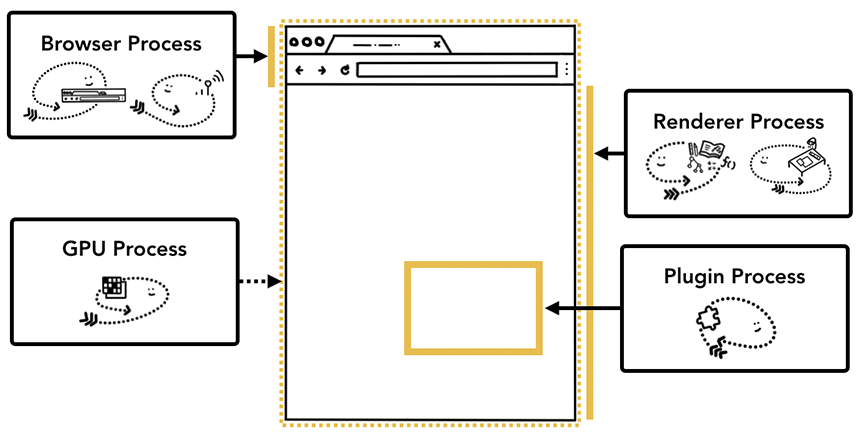
\includegraphics[width=13cm]{kththesis/Figures/chrome_architecture.png}
    \caption[Chrome's multi-process architecture]{Chrome's multi-process architecture \footnotemark}
    \label{fig:chrome_architecture}
\end{figure}

\footnotetext{Source: \textit{Inside look at modern web browser (part 1)} \cite{chrome_architecture}}

Each process also have several threads running at the same time for optimization.

\paragraph{}
Chrome's rendering pipeline \cite{chrome_pixel} contains similar stages as Android's application rendering but with some differences: \todo[inline, color=orange!40]{Emphasize the different stages}
\begin{enumerate}
    \item Parsing: translates the HTML into a DOM Tree.
    \item Styling: applies CSS style to DOM elements.
    \item Layout: computes the geometry of DOM elements (size and position) and produce a layout tree.
    \item Compositing: decomposes the page into layers which can be independently painted and rastered.
    \item Pre-painting: build the property tree to apply to each layer.
    \item Painting: records paint operations into a list of display items.
    \item Tiling: divides the layers into tiles making its rastering less expensive if only a part of it is needed
    \item Rastering: executes the paint operations and decodes images to produce a bitmap.
    \item Drawing: generates a Compositor Frame and sends it to the GPU process.
\end{enumerate}
Every Renderer and the Browser Process can compute frames according the pipeline described above. The GPU process then aggregates all Compositor Frames according to the surface they represent on the screen  and sends calls to the OS's graphics library. For Android, that means pushing a buffer of graphic data to SurfaceFlinger.
\newline
As opposed to Android, the output of the different stages are reused whenever possible and the view is divided so that a small change in the view triggers only a small amount of work to render it. 
For example scrolling only changes the position of a layer. There is no need to go through parsing, styling and layout again, maybe even pre-painting, painting, tiling and rastering if it it was already done.

\section{Problem Analysis}

In the light of the background described above, this sections provides additional motivation and limitations for the research questions. 
\paragraph{}

\textbf{Motivation} \newline
Previous research about Progressive Web Apps performance focused mainly on the performance at start-up (loading time, first paint) but none was found that studied the rendering performance during use. To my best knowledge, this research will be the first to do so.

\medskip
\textbf{Limitations} \newline
As stated above, Android applications and Web Applications on Chrome share two components of the display pipeline (SurfaceFlinger and the Hardware Composer) but differ greatly in the Application Renderer. Thus this research will focus on comparing the smoothness of Android applications and Progressive Web Apps in regards to this last component. 


\paragraph{}
This chapter provided the necessary background to conduct this research and additional motivation and limitations. The next chapter will focus on the method of comparison of PWAs and Mobile Applications and the tools used to do so.
    

\chapter{Methodology}
\section{Comparing the Rendering Process}
   

    \subsection{Chrome's pipeline}
    \todo[inline, color=cyan!20]{Describe Chrome's pipeline model and how I came up with it}
    \subsection{Method of comparison}
    \todo[inline, color=cyan!20]{Conclusions on how to compare both pipelines: a) definition of a frame b) benchmark apps used}
\section{Comparing CPU and Memory}
    \subsection{Android and Chrome tools}
    \todo[inline, color=cyan!20]{Describe available tools on Android and Chrome}
    \todo[inline]{Move to Background}
    \subsection{Evaluating Chrome tools}
    \todo[inline, color=cyan!20]{Describe Experiments used to compare Android and Chrome tools, and their results}
    \subsection{Evaluating Emulators}
    \todo[inline, color=cyan!20]{Explain why Emulators are no good for evaluating CPU and Memory}

We will focus on the fluidity of the apps that can be defined with Frame Per Second (FPS) rate.
Thus, we will compare the FPS rate of a Native Android Application and a Progressive Web App, as well as with a benchmark consisting of : 
    - an app displaying different image/texts every 16/17ms
    - an app with more effort on the CPU : modification of the same pictures/texts or new pictures/texts generated randomly.
\newline

We will measure FPS, CPU and Memory usage to see the impact of CPU and Memory usage in the fluidity of the app.
\newline

\subsection{Scripts implementation}
\todo[inline]{Explain your technical contributions}

\iffalse
\section{(Weekly reports)}
\subsection{Comparing Chrome's PWA and Android Frames}
\paragraph{Week 11}
The question now is 1) what counts as a frame for a PWA (especially if we count the Browser frames) and 2) how to compare it to Android frames.
Those questions are closely linked and are difficult to seperate since Chrome's and Android rendering Pipeline are quite different.

To summarize, on one hand Android's pipeline is pretty straightforward and easy to follow : the OS sends VSync signals that depends on the device refresh rate, asking everything on the foreground to render a frame. In response, the UI thread calls Choreographer\#doFrame which handles callbacks for input, animation before doing some sizing and layout. The Choreographer then hands what it computed to the RenderThread which issues the draw commands and swap the buffers for SurfaceFlinger.

On the other hand, Chrome's pipeline is much less consistent and depends on a lot of parameters. We know that the VizCompositorThread also calls the Choreographer almost at each Vsync though it stops after the animation callbacks. As it is also the thread emitting 'IssueBeginFrame' events, those events are most likely linked, though I don't know when this IssueBeginFrame event is emitted compared to the Choreographer.

Thus, it is meaningless to compare Chrome's frames with Android's from the start of Choreographer or the start of Vsync.

Another point against doing this is the the input events. Those are always handled on Android inside the Choreographer, just before computing the frame. On Chrome, however, they are handled asynchronously and thus an input can affect a frame currently being drawn or start a new one.

This leaves us with comparing the amount of time they spent on computing the frame. For Android, it starts with traversal, and can be accessed with the PerformTraversalStart timestamp. For Chrome, it is a little more complicated as a 'frame' for Android, that is a Buffer Swap, consists of several frames computed in parallel on Chrome's Pipeline.

For a Basic frame which reuse a Main frame already drawn, I believe the computation starts inside ProxyImpl::ScheduleActionDraw. For a basic frame with a new Main frame, it should start at 'BeginMainThreadFrame' event. 

As a Buffer swap consists of both a Basic frame and a Browser frame, and a Browser frame can trigger a Buffer swap by itself, the question is do we count them as part of the PWA's frame or not. If, as I suppose, the Browser frame displays things like the scrollbar, I believe we should count them as a PWA's frame as these displays are usually handled by the app on Android. 

Thus, the most meaningful comparison, in my opinion, is the time between the timestamps PerformTraversalStart->FrameCompleted on Android and PrepareToDraw/BeginMainThreadFrame(if new main frame)->FrameCompleted of the Compositor frame of the Browser frame on Chrome (depending which took longest for the corresponding Buffer swap).

\paragraph{Week 14}
Since a frame on Chrome can take different paths depending on the work done (Main Frame/ Basic frame), it would be more meaningful to compare Android and Chrome depending on the path the frames take (ie Main frame/ Basic frame). Thus, it would be most relevant to have one benchmark application displaying mostly Main frames and the other displaying mostly Basic frames.

I read more about Chrome's Graphics to understand exactly what work is done inside a  Main frame and what work is done inside a Basic frame. As Chrome's Graphics have a lot of pending projects to improve it, not all of them are also done on Android, and the documentation isn't always clear or up-to-date, it is difficult to really understand what happens inside a Main frame or a Basic frame's pipeline.

What I do know is that:

    - during a Main frame is computed (not compulsory for each frame) parsing (HTML into DOM), style (apply CSS), layout (DOM elements relative to each other) and possibly paint setup, which converts the DOM into a DisplayList, similar to a texture.

    - painting (converting that texture into a bitmap of pixels) and compositing (assembling layers into one image) are done by the compositor (broadly speaking, seems to contains several threads)

Chrome's Graphics teams try to remove as much work as possible from the main frames, as they are block the UI thread. Thus, anything that represents simple texture manipulation is done entirely by the compositor. This is true for scrolling (since the main frame computes more displays than what is currently rendered on the screen) and other CSS style effects (though I don't know which one).

For the 'Basic path' benchmark app, I suggest a simple one that just scrolls a big list of items (text, images... yet to be decided).

For the 'Main path' benchmark app, the one I currently have which just changes texts every few ms is sufficient, though we can change the content to display to match the content from the other benchmark app.




\subsection{Measuring Tools Android app}
\paragraph{Week 1}
 There are not many tools available to profile Android applications aside from Android Profiler \citationneeded. Some other android profilers were developed for research papers but they are mostly unavailable or focus on energy consumption. Android Profiler itself is not suitable for automatic measures as its data can only be viewed in charts and it can impact the app's performance quite a bit (my testing app freezes after 1-2h when using Android Profiler).

    Thankfully, it is possible to with command-line tools such as adb and dumpsys. Thus, I can access : 
            - the jank rate of an app with 'adb shell dumpsys gfxinfo <package-name>' which shows several statistics about the application frames since recording. Those statistiques can be reset by adding 'reset' to the command line. 
            - the memory usage of the application with '<adb shell dumpsys meminfo package-name>' which takes a snapshot of the memory and the time of execution and shows the precise amount of memory used (Proportional Set Size, Private Dirty, Private Clean, etc) in Kb. 
            - the CPU usage of the phone with 'adb shell dumpsys cpuinfo' which reads information from /proc/stats (similar to file /proc/stats in Linux) and shows the \%core-capacity used by each package. However, the information is only updated every five/fifteen minutes so it will not be possible to do short experiments.
\paragraph{Week 2}

\todo[inline]{Add repo link, this is a technical contribution for example}
I have written a script with monkeyrunner to automatically gather data (fps, cpu, memory) when using an app.The script launches the app and gathers data (total frames rendered, janky frames, cpu usage, PSS memory) every 5 min (the cpu usage info gets updated every 5min only) and 10 times during the experiment before killing the app. This experiment is done 10 times on a device.

\paragraph{Week 5}
The command 'adb \todo{What is adb?} \citationneeded shell top -n 1' is more suited for measuring \%CPU as it is computed from the time of the last top frame rendering (i.e. last command in this case) thus giving a better control over the measurements.

\paragraph{Week 6}
The command top and dumpsys cpuinfo give really different results.
the results from cpuinfo and top are a lot different. I assume it is because cpuinfo shows \%CPU core capacity and top only the \% total CPU capacity. Apparently, top is also less accurate than cpuinfo as it makes some estimations.
%https://stackoverflow.com/questions/40494189/top-command-vs-dumpsys-cpuinfo-which-one-is-more-accurate.
\textit{dumpsys cpuinfo}: reads the ticks/jiffies spent in user mode and kernel mode (kernel + user = cputime) during a time interval (from SystemClock.uptimeMillis()), converts the jiffiesMillis to milliseconds. Gives us the \%cpu core (next to package name).
%Sources :
%    https://linux.die.net/man/5/proc,
%   https://github.com/aosp-mirror/platform_frameworks_base/blob/master/core/java/com/android/internal/os/P    rocessCpuTracker.java,
%   https://stackoverflow.com/questions/40186347/dumpsys-cpuinfo-in-android-interpreting-the-results-of-thi    s-command
\newline
\paragraph{Week 7}
%https://github.com/aosp-mirror/platform_system_core/blob/nougat-release/toolbox/top.c
\textit{top}: gives the \% of ticks spent in user and kernel mode for the package over the total number of ticks during the time interval, in other words the \%CPU total without any estimations. As I thought, there is no way to change the change it to \%CPU core

Since PWAs have a specific process to use the GPU, is it the same for Android ? How does gfxinfo gets its information ? Is it the packages that does the rasterization, etc ?
%https://github.com/aosp-mirror/platform_frameworks_base/blob/nougat-release/core/java/android/view/WindowManagerGlobal.java
\newline
TODO: \textit{Find gfxinfo source code. I already have the last part but I am still missing the most important: the first one}

\paragraph{Week 8/9}
I started to analyse the systraces from a native app and a PWA, and read about Android Graphics pipeline. You can find the systraces on Google Drive. Here is what I understand so far (though some if it might be just guessing from the systraces) : 

The baseline of the display pipeline is divided between the app rendering, SurfaceFlinger composition and the Hardware Composer (HWC). The app communicates with SurfaceFlinger through a BufferQueue containing buffers of graphical data. When an app wants to render something on the screen, they execute their rendering process and call the BufferQueue to submit their graphical data (dequeue() to retrieve a buffer of BufferQueue, queue() to return it). At each Refresh Display (once every ~16/17ms), SurfaceFlinger wakes up and process the buffer waiting in BufferQueue, or goes back to sleep if there is none. 

Apparently, SurfaceFlinger processes differently a native app and a Chrome PWA though the difference is not visible on the systrace. When a buffer is available, SurfaceFlinger collects the buffer, then asks the Hardware Composer how to perform composition, that is which layer SurfaceFlinger composites before handing the buffer to HWC. HWC handles all the rest. For a 'normal' app, SurfaceFlinger first composes buffers to an onscreen surface, and then the surface gets composited on the screen. Chrome uses instead a 'SurfaceView' which allow SurfaceFlinger to directly composes buffers to the screen.

Ideally, to study the difference of smoothness between a PWA and a native app, this difference would have to be studied too. However, it would certainly require experiments similar to the ones done in Benchmarking Handheld Graphical User Interface: Smoothness Quality of Experience    with a camera measuring the time elapsed from the user input to the actual display on the screen, but I have neither the equipment, nor the skills to do them. 

Thus, I will focus on the first part of Android display pipeline : the app rendering. Please look at the systraces to understand more easily the following explanation.

For a native app, everything is done on the same process though on different threads (UI thread and RenderThread). A frame, as it seems to be defined by systrace (enter 'M' after selecting the frame (the 'F' circle) to see), starts when Choreographer{\#}doFrame wakes up, and ends when the queue() call finishes. Thus, it can be defined as the time taken to make the buffer available to SurfaceFlinger. I assume this is also the time considered by dumpsys gfxinfo to separate good frames from janky ones.

\paragraph{Week 9}
For an app using Android's framework, it is possible to get the frames timestamps (frames from the last 2s, using the flag 'framastats' with dumpsys gfxinfo). By studying Android's source code, I was able to link the systrace events with the timestamps.
\newline
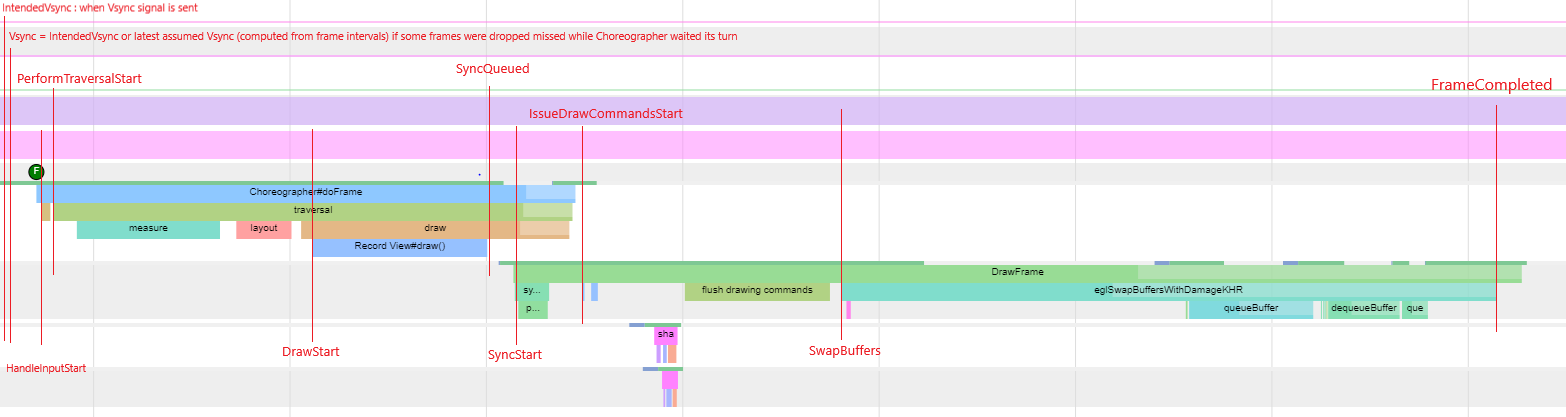
\includegraphics[width=13cm]{kththesis/Android_frame_timeline.png}
            
\subsection{Measuring PWA Tools}
\paragraph{Week 1}
Progressive Web Apps are difficult to profile. The only tools available are Lighthouse in Chrome and WebPageTest, which doesn't measure any of the desired metrics, as well as the developper Tools.

The Developper Tools in Firefox and Chrome can give us the average fps rate (with a script in another Developer Tools window for Chrome thanks to this post : https://stackoverflow.com/questions/48079661/how-to-get-the-average-fps-in-chrome-devtools) and a chart of CPU and Memory usage. We can also download the recording in a JSON file (a list of the threads as I understand it). I have tried getting the CPU or Memory usage from this JSON file or in a similar manner as the fps rate, but I haven't succeeded yet. 

I also thought of using the same dumpsys command-line tool as native applications to measure PWAs performance, for example by looking the browser app or by searching the packet associated with the PWA. To test this,  I looked at the total number of frames rendered by each package while only displaying and interacting with a PWA. However, the results were not conclusive as the package com.android.chrome increased slowly (less than 100 frames after several minutes of interaction) and others faster (see comments) %(NavigationBar0/android.view.ViewRootImpl@6548de3 with around 300 frames and StatusBar/android.view.ViewRootImpl@5cdc3e0 with around 500 frames)%
. 

I have also discovered it is possible for a Progressive Web App to have a WebAPK if downloaded with Chrome, thus making it possible to measure Progressive Web App's performances with the same tool dumpsys as a native application. However, this complete installation of PWAs are still not available on other browsers, and I have not been able to truly install a PWA on Android Emulator yet to test this. I might have to implement one myself. 
\paragraph{Week 2}
 A script (that can also be found in the Script repository) can be used in the Dev Tools' Dev Tools (which I call devception in short) to compute the average FPS rate, CPU usage and Javascript heap from a profile recording.

The Javascript heap can be compared to the Java heap measured in android applications, but doesn't reflect the total memory used by an application. Unfortunately, this is the only memory use measured by Chrome performance profiler. We could also access chrome memory info in the same way as the other android apps, but it might contain memory not used by the Progressive Web App.
\newline
TODO: 
\textit{See if we can classify the memory not used by the pwa, for example with a minimum pwa and another from the benchmark}
\paragraph{Week 3}
For the progressive web apps, I looked at webdrivers like appium/webdriverio. It is possible to record traces with them, but the tracing is periodically stopped by ChromeDriver to avoid filling the buffer completely, then restart at some points durint the test. There are no methods to control the start and stop of the tracing.  

I also looked at Chrome Devtools Protocol (send over websockets) which has an experimental Tracing domain able to completely control the trace. I used it with the python library tri\_cdp and am able to automatically get trace logs renderable in the Chrome Devtools Timeline. The script and the trace logs (from the trio\_cdp tracing and timeline tracing for comparison) are in the Script repository. 
Unfortunetaly, as it is an experimental domain, it can be removed at any time. If that happens, I will probably have to do the experiments manually.

Finally, I have downloaded and looked at Chrome Devtools source code in order to understand how they compute the cpuTime and frames from the raw events.
\paragraph{Week 4}
I have looked at Chrome Devtools source code, copied and adapted the necessary class and functions in order to retrive the same models computed by Chrome devtools. The scripts (extractFromTrace/extractData.js) are on the Git repository. I can now compute the FPS, CPU\%, and Memory usage from the trace just like I do on Chrome devtools.

However, I noticed on the PWA's traces attained by Chrome remote debugging that there is no cpuTime value (from which I usually extract the CPU usage), but Chrome Devtools do show a CPU usage graph. To be clear, this is just for traces done by Chrome Devtools in remote debugging mode. The traces attained from a PWA by the python scripts are complete and can be processed into CPU times. However, there might be some other things to take into account aside from the CPU time, so I will look more into Chrome Devtools source code to find out.

\paragraph{Week 5}
CDP' SystemInfo.getProcessInfo could get us the cpuTime of each process since running, but calling throws an error ('Not found'). Bug reported on 11 Dec. 2018. No visible progress since then. 

How they draw the CPU Overview graph on Chrome Timeline (from what I understood)
   They consider a small time interval of the recording which represents, let's say, 4px on the screen. The cpu usage is represented vertically by the cpu time used during this interval. So for example, 100\% cpu usage during this interval would be represented by a square of 4px by 4px. 50\% by a rectangle 2px high, etc.  For each event running during this time interval (its start and/or end time is between the start and end time of the time interval), the time the event spent inside that interval is added to the rectangle. So an event running 50\% of the time interval would add 2px to the height of the rectangle and so on for each event. 

Thus, the CPU Overview graph isn't a true representation of the CPU usage as it doesn't take into account functions waiting for something, juste the start and end time of events. 

How and why they compute the CPU time of frames
    How you might have guessed from the previous explanation, the cpuTime computed for the frames isn't used at all to draw the CPU Overview. It is for the user to have an idea of how much time is spent in the frame processing instructions (at least instruction events). It is roughly the selfTime sum of events from the main and compositor threads. 

Solution
    Fortunately, Chrome does track CPU usage with a CPU sampling method from which we can compute the total time the CPU is not idle, thus giving a good estimate of the CPU usage.
This solution also gives more reasonnable results (40\% core CPU as opposed to 114\% core CPU with the CPU time for a really janky PWA).

CPU Sampling explanation here : https://devblogs.microsoft.com/devops/how-cpu-sampling-works/

\paragraph{Week 6}
Since Chrome devtools only keeps track of the Javascript heap, it is necessary to classify the memory used by a PWA in order to compare it to the memory used by a native app.
To this goal, I ran in succession : the empty PWA, the android app benchmark with the empty PWA installed but killed, the benchmark PWA, the android app benchmark with the benchmark PWA still installed but killed. I made sure chrome was not running. Logs were saved every minute (10 times) from dumpsys meminfo as well as cpuinfo, gfxinfo and top in order to test them on a PWA. 

As for the memory usage, I am not quite sure what to make of the results yet.
4 packages appear on the foreground (Foreground section of meminfo) when running a PWA : com.android.chrome, com.google.android.gms.persistent,  com.android.chrome:privileged-process and com.android.chrome:sandboxed-process when there is only one with a native app. The package org.chromium.webapk also appear either on the Previous or the Cached section but it doesn't use any CPU.
These packages disappeared when killing the empty PWA, but not when killing the benchmark PWA though they hardly used any CPU after (only com.google.chrome which uses 0.2-0.3\%CPU core). 
I will probably do more similar experiments and research more about what memory should be used to help compare the fluidity of PWA and native apps.

Lastly, there is also an inconsistency with the CPU usage of PWAs. With the CPU sampling of Chrome devtools, I have around 4\% CPU usage with the benchmark PWA. But looking at the entire CPU usage of the phone when running it, I don't understand where this number comes from. I will also have to research more about it and how the work of the PWA is divided between the different packets.

\paragraph{Week 7}
3 different processes run when a pwa is running : the Browser, the Renderer and the GPU Process. It is the same as a Chrome window on a desktop. Usually (unless not enough ressources), each tab on a Chrome window has its own Renderer process. It is the one where the website/PWA is truly running. Each tab has its own Rendererer process both for security (one tab cannot access information from another tab opened) and performance (one tab crash doesn't impact the other tabs). The GPU Process is here for security as a middle-man between the tabs and the system's 3D API. It's probably the reason why Chrome's frame aren't detected by dumpsys gfxinfo. I'm not sure yet what exactly the Browser process does.

The \%CPU computed with the trace not coherent with the \%CPU measured by dumpsys.

I changed the code to not count idle frames when computing frame rate. 
\newline

\paragraph{Week 8/9}
As you might remember, Chrome instead uses 3 different processes : the Renderer (com.android.chrome:sandboxed\_process), the GPU Process (com.android.chrome:privileged\_process) and the Browser. All the rendering part seems to be done by the Renderer while the communication with SurfaceFlinger is done by the GPU Process (CrGpuMain thread). To define a frame, Chrome devtools only consider events from the Renderer process, with a frame ending when a new one starts.

Thus, we need somehow the time it takes for the GPU process to queue the buffer to really compare the frame times of a native app and a Chrome PWA. However, the GPU Process calls don't seem to follow Renderer calls that closely. It might also be what Chrome calls the 'housekeeping work' in https://developers.google.com/web/fundamentals/performance/rendering and advice to 'finish the work' in under 10ms instead of 16.6ms

\paragraph{Week 9}
As for Chrome, I first thought that the 'GPUTask' events matched the events showed on systrace (dequeueBuffer, queueBuffer and eglSwapBuffersWithDamageKHR). I counted the number of frames and GPUTask events on the 500 traces I did for the single-cpu experiments. They had a correlation coefficient of 0.99971 so I though it truly matched.
However, I did some another trace to check this theory but this time interacting with the PWA with a button. The number of GPUtask events was far below the number of frames (220 GPUTask << ~500 frames) while there was always 2 or 3 GPUTasks for each frames in all the 500 traces.
Fortunately, I discovered another 'trace' tool available through chrome://inspect/device{\#}devices that presents all the trace events in their visual timeline, as opposed to Chrome Devtools. By turning on the 'gpu' category, an event called 'GLES2DecoderImpl::DoSwapBuffers' which calls 'NativeViewGLSurfaceEGL::RealSwapBuffers' appears. I think it's safe to assume they correspond to Android's 'eglSwapBuffers' which marks the end of the frame.

However, the number of SwapBuffers event doesn't always match the number of frames as computed by Chrome Devtools. I made 9 experiments with different clicking speeds (the traces and spreadsheet are on Google Drive). They do match when there is no clicking, but the difference seems to increase the more interaction there is.

\paragraph{Week 10}
The VizCompositor thread on the GPU Process seems to be the one scheduling the frames similarly to Vsync signal on Android: it has an event Graphics.Pipeline with args.step = 'IssueBeginFrame' which is linked to the Scheduler::BeginFrame in the compositor thread (Renderer Process). In most cases, the compositor thread also request a MainThreadFrame from the main thread (CrRendererMain in Renderer process). CrRendererMain computes the main frame (under the event ThreadProxy::BeginMainFrame) and sends it back to the compositor, though the main frame can be aborted at this point. The Compositor thread then makes the necessary preparations to draw the frame, with sometimes help from the GPU Process, and emits a 'DrawFrame' event. The GPU Process main thread takes over and swap the buffers to pass it on to SurfaceFlinger.

It is easy to follow a main frame drawing on the compositor and renderer main thread as ThreadProxy::ScheduledActionSendBeginMainFrame, ThreadProxy::BeginMainFrame and other events inside ProxyImpl::ScheduledActionDraw (which emits 'DrawFrame') have the same id/number in begin{\_}frame{\_}id or 'source{\_}frame{\_}number' args. It is a little trickier to follow it on the GPU Process, especially since the SwapBuffer events don't always follow closely the 'DrawFrame' event, but since there is always almost as much Swapbuffers as DrawFrame event (there can be 1 or 2 more DrawFrame than SwapBuffers in the frame{\_}viewer experiences I made), but it shouldn't be too much of a problem.

However, some main frames are drawn several times in a row, and only when there is some user inputs. I suspect it is because they only need to alter the style of the main frame to display the animations triggered by user input.

\paragraph{Week 11}
I have done some progress regarding Chrome's graphics pipeline and can now detect when a new frame started and was completed.
As you know, I build a first model from a manual inspection of different PWA traces (with different events depending on the categories selected during the trace). I tested this first model with a script which extracts the frames from the trace events and raises an error whenever something is not as I expected. Whenever an error was raised, I looked at the trace and either debugged my script or adapted my model. This was done until no unexpected errors was raised.
\newline
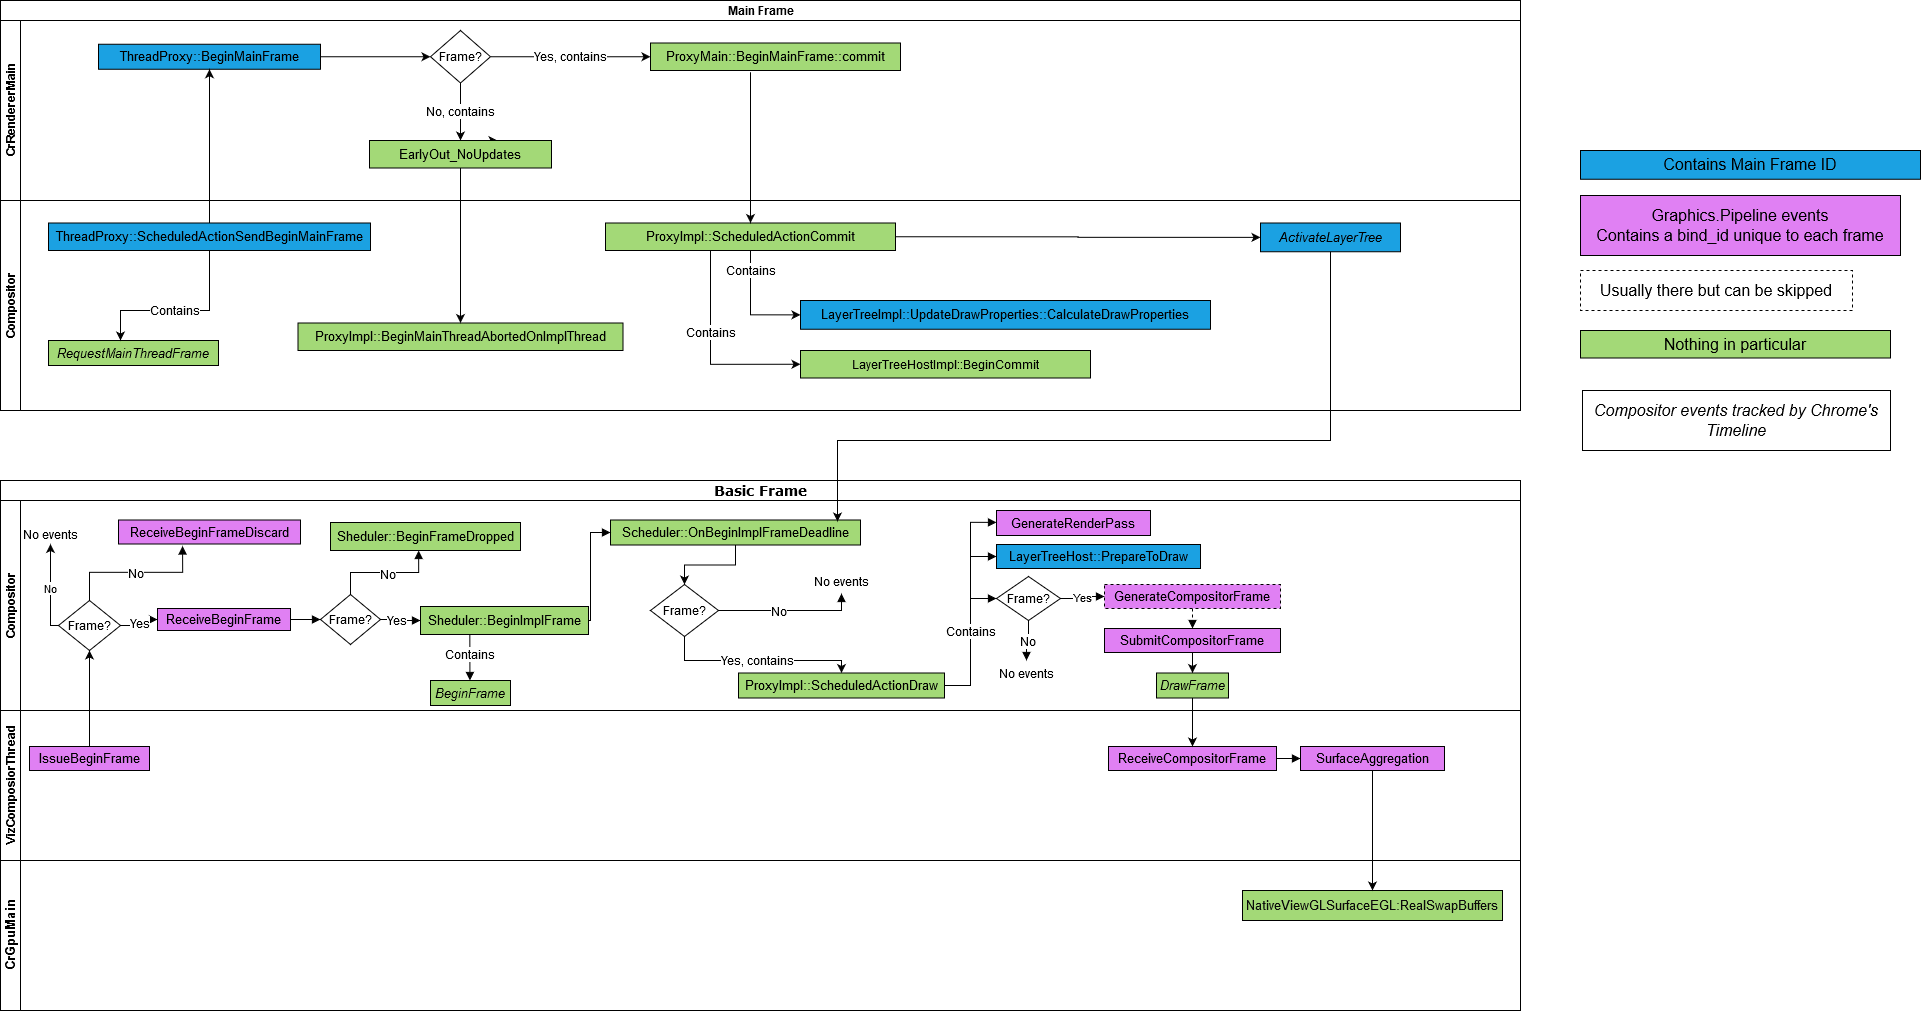
\includegraphics[width=13cm]{kththesis/Chrome_Graphics.png}
\newline
All events linked to the computation of a frame are not tracked (for example, the rasterization or tiles manager are not). I track only the events related to the completion or cancellation of a frame.

Note that there are two kinds of frames:
    - the 'Main' frames which, as I understand is the core structure of the frame and is recomputed whenever something changed in the javascript.
    - the 'Basic' frames which is the path followed by every frame that is rendered. Several 'basic' frames can share the same main frame when there is only a small difference between them, for example in the CSS (my guess is it happens when only the CSS or the scrolling position changes, cf the previous email).

Also note that those two frames are computed in parallel, and do not wait for each other. Usually, the Compositor asks for a main frame inside  Scheduler::BeginImplFrame, but it might also happen later in the pipeline. The main frame can also be committed and activated too late, and thus the basic frame pipeline is re-started after the main frame was computed.

Please tell me if there is anything you don't undertsand, or if you would rather have me explain it via Skype or Zoom.

I am pretty confident in my model but I still have to test it with scrolling.

There is also another problem. In some of the manual clicks traces (traces 3, 4, 6 and 8), some basic frames are computed from the Browser main thread instead of the Renderer process/Compositor thread and then linked to every following SurfaceAggregation events, resulting in a a snowball of errors in my script. As a web app is only run inside a Renderer process for security, I suspect this browser frame is actually the small window that sometimes pop-up on top of the app asking if I want it translated, though I don't really remember it from the experiments. I will try to reproduce this examine it further.

\paragraph{Week 12/13}
The following model was build from several experiments from my PWA benchmark app with diffferent user interactions (automatic clicking every 20, 100, 300, 500, 1000ms, manual clicking, refresh, nothing) and scrolling from another PWA (https://pwa.rocks/). I intend to do more experiments from other PWAs to further validate my model and not have any surprise later in the thesis.


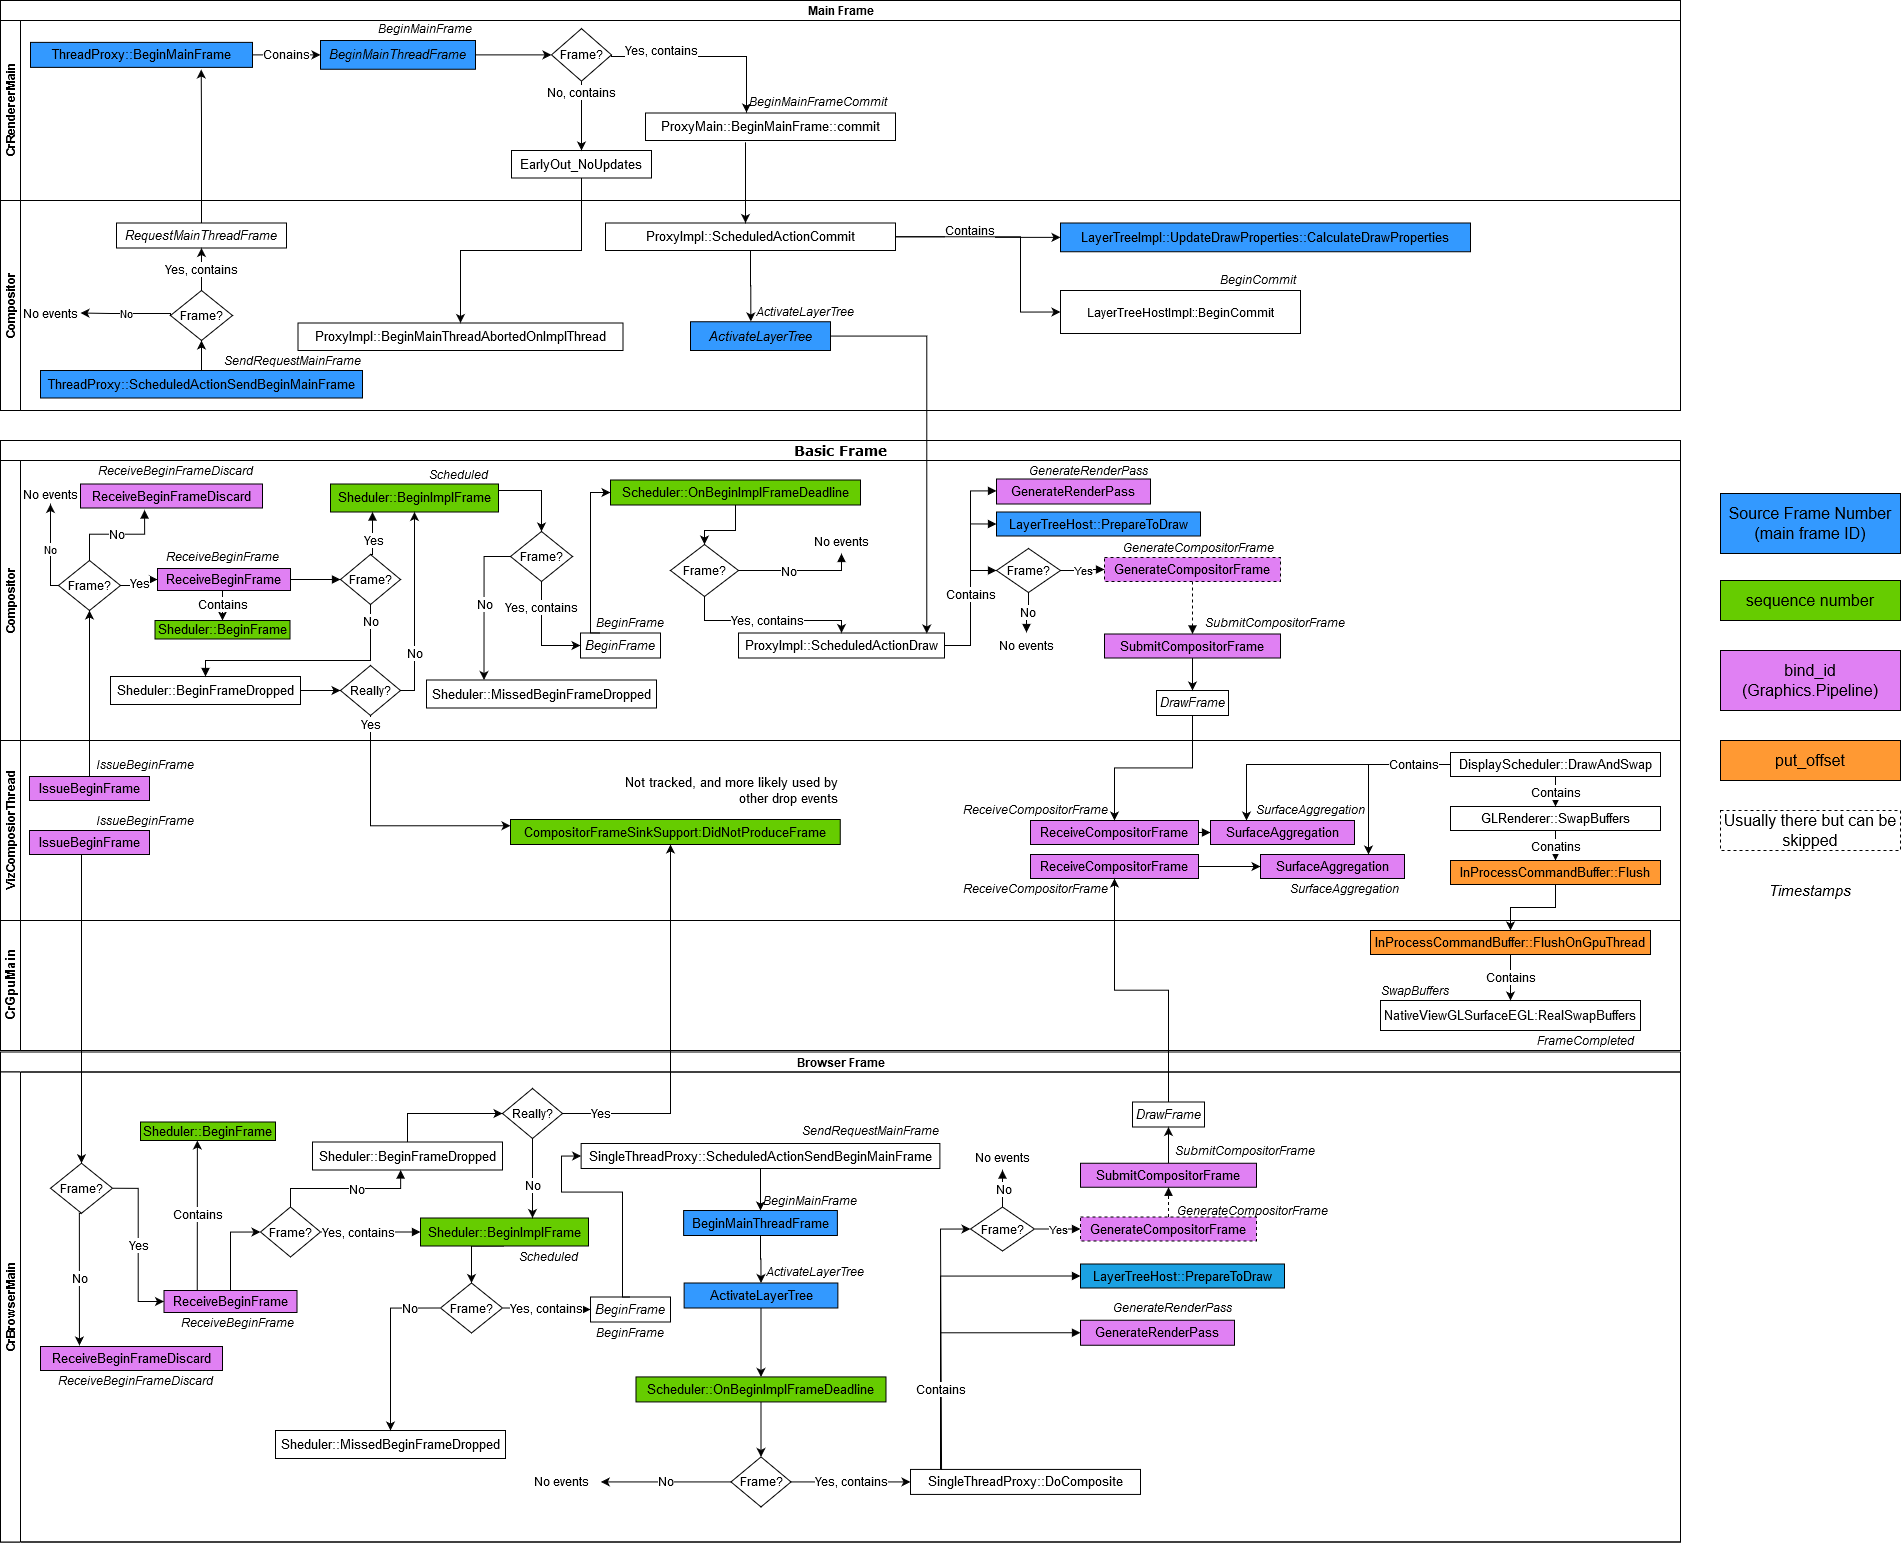
\includegraphics[width=13cm]{kththesis/Chrome_Graphics_v2.png}
\newline
As you can see, I differentiate 3 types of frames : the Compositor frames, the Main frames and the Browser frames.
As I explained before:
    - the Main frames are the core sctruture of every PWA's frames and are recomputed whenever something changes in the javascript.
    - the Compositor frames, or basic frames is the path folloxed y every PWA's frames. Some Compositor frames may share the same Main frame if the difference can all be handled by the Compositor thread.
    - the newly added Browser frame represents, I suspect, everything displayed by the browser in itself and not the app, for example the addressbar, the little scroll bar or the refresh animation.

When Chrome swaps buffers to send it to Android's SurfaceFlinger, it actually sends 2 frames : one Compositor frame and one Browser frame which are probably combined into a single surface by the 'SurfaceAggregation' events, or somewhere near. Only one frame change is necessary to trigger a SwapBuffer. While the Compositor frame is usually always changing, it is not always the case and the Browser frame alone can change between two following SwapBuffers. In my previous experiments from which I built the previous model, the browser didn't displayed anything, and thus the Browser frame was always the same and didn't appear.

Some side notes about the workflow :
    - I noticed some of the supposedly dropped Browser Frame actually continued on the rendering path. This seems to be the case when there is no aknowledgment of the dropped frame on the VizCompositorThread (CompositorFrameSinkSupport::DidNotProduceFrame event). But, as the sequence number used by this event to identify the frame is the same for both Compositor and Browser frames and sometimes the event can be a little late to turn up, I find it easier to just recover the recover the dropped frame than follow this event. 
    - the put\_offset which I use to link frames to SwapBuffers is actually not unique to each draw but some time elapses between the reuse of a put\_offset so it is easy to know which frame is beaing drawn
    -  I did not put this in the workflow, but sometimes during a refresh, a MainFrame is defered: ThreadProxy::BeginMainFrame contains nothing except except for an EarlyOut event, and the frame will be computer after the next main frame request. However, this causes a mismatch in the following frames between the main frame id requested (the one inside SendBeginMainFrame and ThreadProxy::BeginMainFrame) and the main frame's id actually computed (all following events).


On another note, I also have a small concern. I did some other android systraces when doing a refresh of PWAs and was surprised to see a lot of complete Android frames from Chrome's package. This could invalidate my hypothesis of the Browser frames representing what the browser displays for itself. However, this doesn't happen on a scroll so I am puzzled by what those Android frames are. 

Nevertheless, I don't think we should count them as PWAs frames as those doesn't happen apart from refresh events. 

\subsection{PWA development}
`\paragraph{Week 5}
Regarding PWA development, I had started it Angular.js but I found this website (https://hnpwa.com/) which compares the same PWA on different frameworks and different implémentations. I filled a spreadshit (Script repository/data) with implementations on Angular, React and Preact (since I am already familiar with their API) and other impressive ones to more easily compare them. 

From this data, Angular doesn't seem a good choice to develop a performant PWA. The one done without framework is by far the most performant, but most of web apps now are too complicated to developp without a framework, and thus it will not be realistic. Polymer and Viper also had good performance, but there wasn't any other implementation and I am not familiar with it. Thus, React and Preact are a better choice. Preact was chosen in the end because it is lighter than React, keeping in mind the limited memory space available on smartphones. 

\paragraph{Week 6}
Even though Preact should be 100\% compatible with React, it seems there are still some issues left, especially with material-ui and react-redux libraries which are the most common libraries used in React and still do not have a complete equivalent on Preact. Thus, I will actually develop it in React (and maybe see the compatibility with Preact)


\subsection{Emulators}
\paragraph{Week 2}
As Xamarin Android Player is now deprecated, I don't think it is a good idea to use it (and the download links on the GitHub page is not working). Bluestacks aims to be faster and more performant than  a real device, and thus is not suitable for this research which needs real device emulator. Genymotion is faster to start than Android Emulator but seems to have higher janky rates than it. I will do some experiments to properly compare their performance compared to a real device, and eventually other emulators.

\fi


\chapter{Results}
\subsection{Emulators}
I have finished the experiments on Genymotion, and the numbers are too different to make future experiments on Genymotion (52 FPS, 72\% CPU, 72MB for real Samsung S6, 32FPS, 29\% CPU, 24MB for Genymotion). I started the experiments on Android Emulator (by downloading a Samsung Galaxy S6 skin and setting appropriate settings) but the first results don't seem promising either (FPS vary from 25 to 59 FPS, 13-25\% CPU and 16-50MB).

\paragraph{Week 7}
The experiments are finished and every emulators have too different results from real devices to use them. 
Results available on Google sheets.

\subsection{PWA Measuring tools}
\paragraph{Week 8}
To understand what Chrome's Devtools exactly measures as \%CPU, experiments were done on a single-core emulated device running PWAs with different CPU workloads (different DOM changing speed). CPU usage was extracted by :
    - dumpsys cpuinfo for each process (Browser, GPU, Renderer)
    - CPU time as computed by Chrome devtools
    - \%CPU as computed from Chrome CPU sampling
The first experiment was done with 10 measures for each workload, and the second one with 100 measures for each workload.

The results from Chrome Devtools, either from the CPU time or CPU sampling don't come close enough to results from dumpsys cpuinfo, used for Android apps. Thus, it is not possible to use Chrome's Devtools CPU measures to compare PWAs and Android apps

\chapter{Discussion}
\blindtext

\todo[inline]{Include future work and limitations of this thesis}

\chapter{Conclusions}
\blindtext

\listoftodos{Notes}

\listoffigures
% Print the bibliography (and make it appear in the table of contents)
\printbibliography[heading=bibintoc]

\appendix

\chapter{Something Extra}

% Tailmatter inserts the back cover page (if enabled)
\tailmatter

\end{document}
